\documentclass[a4paper,10pt]{article}

\usepackage{ucs}
\usepackage[utf8]{inputenc}
\usepackage{amsmath}
\usepackage{amsfonts}
\usepackage{amssymb}
\usepackage{amsthm}
\usepackage{caption}
\usepackage{subcaption}
\usepackage{hhline}
\usepackage[english]{babel}
\usepackage[T1]{fontenc}
\usepackage[pdftex]{graphicx}
\usepackage{ stmaryrd }
\usepackage{fullpage}
\usepackage{multirow}
\usepackage{enumitem}
% \usepackage{hyperref}

\usepackage{tikz/tikzit}

\title{1D DG method}
\author{Etienne PEILLON}
\date{15/05/2019}

\begin{document}
 \maketitle
 
 \section{Problem}
 
 We consider the following problem:
 
 \begin{equation} \label{eq:initial}
  \alpha u - \mu \Delta u = f
 \end{equation}

 on the interval $\Omega = ]a,b[$ with one of the three following boundary conditions:
 \begin{itemize}
  \item Dirichlet conditions: $u(a) = u_a^D$ and $u(b) = u_b^D$;
  \item Neumann conditions: $u'(a) = u_a^N$ and $u'(b) = u_b^N$;
  \item Mixed conditions: $u(a) + \gamma_a u'(a) = u_a^M$ and $u(b) + \gamma_b u'(b) = u_b^M$.
 \end{itemize}

 \section{Discontinuous discretization}
 
 To discretize the problem we will follow some step:
 \begin{enumerate}
  \item weak formulation of the problem compatible with the method
  \item writing of the basic matrix
  \item implementation
 \end{enumerate}
 
 The goal of this report is simple: give a little overview of the DG method with understandable but 
extendable notations.

 \subsection{Weak formulation}
 
 Let be a subdivision $a = x_0 < x_1 < \dots < x_{K-1} < x_K = b$ of I. We write $C_n = 
]x_{n-1},x_n[$, so that we have $K$ cells, and $\mathcal{E}_h = \{ C_n \}$ where $h = \max 
\limits_{n} |C_n|$. We also note $h_n = |C_n| = x_n - x_{n-1}$.
 
 We consider the broken Sobolev space, highly depending on the subdivision of the domain (see 
Riviere):
 \begin{equation}
  H^1(\mathcal{E}_h) := \{ v \in L^2(\Omega) \quad that \quad \forall E \in \mathcal{E}_h, v|_E \in 
H^1(E) \}
 \end{equation}

 Denote that $H^1(\Omega) \subset H^1(\mathcal{E}_h)$.
 
 \paragraph{}
 The strong idea of discontinuous Galerkin method is to approximate the problem, not with an 
approximation of $H^1(\Omega)$ as for continuous Galerkin method, but with an approximation of 
$H^1(\mathcal{E}_h)$.


\paragraph{}
Let be $v \in H^1(\mathcal{E}_h)$, and multiply \ref{eq:initial} by it and then use Green formula 
(also known as integration by parts in 1D). We take care that Green formula works only on each cell:

\begin{equation}\label{eq:weak}
 \sum \limits_{n=1}^K \int_{C_n} (\mu \nabla u \nabla v + \alpha uv) d\omega - \int_{\partial C_n} 
\mu \nabla u \cdot \mathbf{n}\ v\ d\gamma = 
\sum \limits_{n=1}^K \int_{C_n}  f\ v\ d\omega
\end{equation}

Here exists different methods in the literature. In Riviere, terms are added to create a bi-linear 
symmetric coercive and continuous form on left side and a linear conituous form on the right side, 
so that you can prove existence and uniqueness with functional analysis theorems. The approach is 
very interesting in the theorical way, but complicated for just a simple implementation.

On the other hand, you can use the following approach, which is less general, but more 
understandable as first view of the subject:

\paragraph{}
Because $v \in H^1(\mathcal{E}_h)$, we assume $u \in H^1(\mathcal{E}_h)$ for the resolution of the 
problem, but we want equality of the solution on the common edges of each cell, wich means we have 
a bad-defined value at $u'(x_n)$ in our case, wich is the \emph{numerical flux}.

A solution consists on assuming numerical flux equals one unique value on cell frontiers:

$$
\widehat{\nabla u(x)} \cdot \mathbf{n} = \beta \frac{\llbracket u \rrbracket}{\overline{\Delta x}} 
+ \overline{\nabla u(x)} \cdot \mathbf{n}
$$

where 
\begin{itemize}
 \item $\llbracket u \rrbracket = u^-(x) - u^+(x)$, $u^-$ is the interior value and $u^+$ is the 
exterior value,
\item $\overline{\nabla u(x)} = \dfrac{\nabla u^+(x) + \nabla u^-(x)}{2} $ with the same policy,
\item $\overline{\Delta x} = \dfrac{{\Delta x}^+ + {\Delta x}^-}{2}$ with the same policy.
\end{itemize}



\paragraph{TRUE section}
\begin{itshape}
 Finally, because $v \in H^1(\mathcal{E}_h)$, we have this equality for each elements:

$$
\int_{C_n} (\mu \nabla u \nabla v + \alpha uv) d\omega - \int_{\partial C_n} \mu \nabla u \cdot 
\mathbf{n}\ v\ d\gamma = \int_{C_n}  f\ v\ d\omega
$$
\end{itshape}


\subsection{$H^1(\mathcal{E}_h)$ discretization}

 $H^1(\mathcal{E}_h)$ discretization is quite similar with the discretization of $H^1(\Omega)$. Let 
be a cell $C_k \in \mathcal{E}_h$, then consider $(\phi_n^k)_{n=0,\dots,N}$ a basis of 
polynomials of degree $N$ on $C_k$. We assume $\phi_n^k|_{C_k^c}=0$.

\paragraph{}
We call $\mathcal{D}_N(\mathcal{E}_h) = \mathrm{span}\{ \phi_n^k ,\ 0\leq n \leq N,\ 1\leq k 
\leq K \}$ the approximation of $H^1(\mathcal{E}_h)$. Then we have to choose the type of basis 
function. Here is some possibilities:
\begin{itemize}
 \item monomial functions,
 \item lagrangian functions,
 \item legendrian functions.
\end{itemize}

Obviously, each basis function is the image of a basis function on a reference element composed 
with an affine map. We call $E$ the physical element and $\hat E$ the reference element, and
\begin{equation*}
 F_E : E \longrightarrow \hat E \qquad \text{and} \qquad  F_E^{-1} : \hat E \longrightarrow  E
\end{equation*}
the affine maps between $E$ and $\hat E$.

Since those maps are affine, we have $|\mathrm{det}(\mathrm{D}F_E^{-1})| = 
|\mathrm{det}(\mathrm{D}F_E)|^{-1} = \dfrac{|E|}{|\hat E|}$.

We also express physical basis functions with reference basis functions with the formula 
\begin{equation*}
 \phi_i^E = \sqrt{\dfrac{|\hat E|}{|E|}}\ \hat \phi_i \circ F_E
\end{equation*}
so that $\|\phi_i^E\|_{L^2(E)}=1$ and $\|\hat \phi_i^E\|_{L^2(E)}=1$.

For 1D case, the reference element will be the segment $\hat E = [-1,1]$. Then 
the affine map will be:

\begin{equation*}
\begin{array}{cccc}
 F_k^{-1} : & [-1,1] & \longrightarrow & [x_{k-1},x_k] \\
            & x & \longmapsto & \dfrac{h_k}{2} x + \dfrac{x_{k-1}+x_k}{2}
\end{array}
\text{ and }
\begin{array}{cccc}
 F_k : & [a,b] & \longrightarrow & [-1,1] \\
            & y & \longmapsto & \dfrac{2}{h_k} \left(y - \dfrac{x_{k-1}+x_k}{2}\right)
\end{array}
\end{equation*}

 With this map, we now just have to describe the basis functions on the reference element to have 
every basis functions we need. So we define the basis functions on the reference element by $\hat 
\phi_n$ for $n= 0, \dots , N$ and then we can write $\phi_n^k = \sqrt{\frac{2}{h_k}} \hat 
\phi_n \circ F_k$

\subsection{discretization on each cell}

In this part, we assume $u \in \mathcal{D}_N(\mathcal{E}_h)$ and it can be decomposed as:

$$
u = \sum_{k=1}^K u^k = \sum_{k=1}^K \sum_{n=0}^N u_n^k \phi_n^k
$$

where $\forall n,k,\ u_n^k \in \mathbb{R}$.


Then we can inject $u$ in the equation \ref{eq:weak}. Then we define $U^k = 
(u_0^k, \dots , u_N^k)^\top$ and $U = [U^1, \dots , U^K]^\top$. The next idea is to project the 
equation \ref{eq:weak} on $\mathcal{D}_N(\mathcal{E}_h)$.

\subsubsection{right term}

The right term of the equation is the easiest part of the discretization: we define $F = [F^1, 
\dots , F^K]^\top$ and $F^k = 
(f_0^k, \dots , f_N^k)^\top$ where $f_i^k = \int_{C_k} f \phi_i^k d\omega$.



\subsubsection{discretization of the mass and stiffness term}

Consider $\int_{C_E} (\mu \nabla u  \cdot \nabla v + \alpha uv) d\omega$, and take $v = \phi_n^E$. 
Then 
we can discretize this integral by

\begin{equation}
 \left( \alpha \mathbb{M}^E + \mu \mathbb{S}^E  \right) U^E
\end{equation}

where $\mathbb{M}^E_{i,j} = \int_{C_E} \phi_i^E \phi_j^E d\omega$ and $\mathbb{S}_{i,j}^E =
\int_{C_E} \nabla \phi_i^E \nabla \phi_j^E d\omega$

\paragraph{Mass matrix:}
Firstly, because we have $\phi_n^E = \sqrt{\frac{|\hat E|}{|E|}} \hat \phi_n \circ F_E$,
\begin{equation*}
 \mathbb{M}^E_{i,j} = \int_{C_E} \phi_i^E \phi_j^E d\omega 
 = \frac{|\hat E|}{|E|} \int_{\hat E} \hat \phi_i \hat \phi_j d\hat \omega \cdot |\mathrm{det} 
(\mathrm{D} F_E^{-1})| 
= \int_{\hat E} \hat \phi_i \hat \phi_j d\hat \omega 
=\widehat{\mathbb{M}}_{i,j}
\end{equation*}
Then we just have $\mathbb{M} = \mathrm{diag} ( \widehat{\mathbb{M}}, \dots, \widehat{\mathbb{M}})$.

\paragraph{Stiffness matrix:} Secondly, we just derivate $\phi_i^E$:
\begin{equation*}
 \mathrm{D}\phi_n^E = \sqrt{\frac{|\hat E|}{|E|}} \mathrm{D}\hat \phi_n(F_E) \circ \mathrm{D} F_E 
\qquad \text{and} \qquad \nabla \phi_n^E = \sqrt{\frac{|\hat E|}{|E|}} {\mathrm{D} F_E}^\top 
\nabla \hat \phi_n(F_E) 
\end{equation*}

\begin{align*}
 \mathbb{S}_{i,j}^E &= \int_{C_E} \nabla \phi_i^E \cdot \nabla \phi_j^E d\omega = 
\int_{\hat E} \nabla \hat \phi_i \cdot ( \mathrm{D} F_E{\mathrm{D} F_E}^\top \nabla \hat 
\phi_j) d\hat \omega \\
&= \left( {\mathrm{D} F_E}^\top \nabla \hat \phi_i , {\mathrm{D} F_E}^\top \nabla \hat \phi_i  
\right)_{L^2(\hat E)}
\end{align*}

Finally, we obtain $\mathbb{S} = \mathrm{diag} (\mathbb{S}^1,\dots,\mathbb{S}^K)$.

\subsubsection{Flux discretization}

In the same way than Armand's report, we define $\mathbb{F}$ as the matrix describing the flux 
part. We also define the bound  term $\mathbb{F}^b$. Those are the most complicated terms, wich will 
be treated here with less generality. But without loss of generality, we can write, for any $E\in 
\mathcal{E}_h$:
\begin{equation*}
 \int_{\partial E} \widehat{\nabla u}_E \cdot \mathbf{n}_E\ v\ d\gamma 
 = \sum_{d=1}^D \int_{\partial E^d} \widehat{\nabla u}_E \cdot \mathbf{n}_E^d\ v\ d\gamma
\end{equation*}
where $\left\{ \partial E^d,\ d=1,\cdot,D \right\}$ are the faces of $E$.

Then we have two cases:
\begin{itemize}
 \item $\partial E^d$ is the frontier between two elements,
 \item $\partial E^d$ is a part of the frontier of the domain $\Omega$.
\end{itemize}
Therefore, we have two treat those two cases distinctly.

\paragraph{If $\partial E^d$ is the frontier between two elements:}

We can make this separation:
\begin{align*}
 \widehat{\nabla u}_E \cdot \mathbf{n}_E 
 &= \beta \frac{\llbracket u \rrbracket}{\overline{\Delta x}} + \overline{\nabla u(x)} \cdot 
\mathbf{n} \\
&= \underbrace{ \left[-\beta \frac{u^+}{\overline{\Delta x}} + \frac{ \nabla u(x)^+ \cdot 
\mathbf{n}}{2} \right]}_{ \text{interior contribution} } 
+ \underbrace{\left[ \beta \frac{u^-}{\overline{\Delta x}} + \frac{ \nabla u(x)^- \cdot 
\mathbf{n}}{2} \right]}_{ \text{exterior contribution} }
\end{align*}

Then, if $E^d$ is the neighbor of $E$ by $\partial E^d$, we have to compute, for all $i,j 
=0,\dots,N$:
\begin{equation*}
 \int_{\partial E^d} \left( - \beta \frac{\phi_j^E}{\overline{\Delta x}}  + \frac{1}{2} \nabla 
\phi_j^E \cdot \mathbf{n}_E \right) \phi_i^E \ d \gamma
\quad \text{and} \quad
\int_{\partial E^d} \left( \beta \frac{\phi_j^{E^d}}{\overline{\Delta x}}  + \frac{1}{2} \nabla 
\phi_j^{E^d} \cdot \mathbf{n}_E \right) \phi_i^E \ d \gamma
\end{equation*}

\paragraph{If $\partial E^d$ is a part of the frontier of the domain $\Omega$:}
We have to consider the bound condition. We assume here this is a Dirichlet condition 
$u|_{\partial \Omega} = g$. That gives us:
\begin{itemize}
 \item $u^- = g$,
 \item $\nabla u(x)^+ = \nabla u(x)^-$ and $\overline{\nabla u(x)} = \nabla u(x)^+$,
\end{itemize}
and
\begin{equation*}
 \widehat{\nabla u}_E \cdot \mathbf{n}_E 
 = \underbrace{\left[ -\beta \frac{u^+}{\overline{\Delta x}} + \nabla u(x)^+ \cdot 
\mathbf{n} \right]}_{\text{flux contribution}}
+ \underbrace{\left[ \beta \frac{g}{\overline{\Delta x}} \right]}_{\text{bound contribution}}
\end{equation*}
Then we have to compute, for all $i,j=0,\dots,N$:
\begin{equation*}
\int_{\partial E^d} \left( - \beta \frac{\phi_j^E}{\overline{\Delta x}}  + \nabla 
\phi_j^E \cdot \mathbf{n}_E \right) \phi_i^E \ d \gamma
\quad \text{and} \quad
\int_{\partial E^d} \beta \frac{g}{\overline{\Delta x}} \phi_i^E d\gamma.
\end{equation*}

\paragraph{}
We assemble all those computations in two matrix $\mathbb{F}$ and $\mathbb{F}^b$.

\iffalse

\paragraph{flux between interior elements}

Let be an interior element, without common component with the boundary. Assuming that the normal 
vector is constant by part, we can cut the integral on each part in $D$ integrals:

\begin{multline*}
 \int_{\partial E} \widehat{\nabla u}_E \cdot \mathbf{n}_E\ v\ d\gamma 
 = \int_{\partial E} \widehat{\nabla u}_E \cdot \mathbf{n}_E\ v\ d\gamma
 = \int_{\partial E} \left( \frac{\beta}{2} {u^+}_E + \frac{1}{2} \nabla {u^+}_E \cdot \mathbf{n}_E 
\right) \ v\ d\gamma \\
+ \int_{\partial E} \left( -\frac{\beta}{2} {u^-}_E + \frac{1}{2} \nabla {u^-}_E \cdot \mathbf{n}_E 
\right) \ v\ d\gamma
\end{multline*}
 We call the first integral the self interaction flux and the second integral the neighbor 
interaction flux.

\subparagraph{self interaction flux} 
Since we have
\begin{equation*}
 \frac{\beta}{2} {u^+}_E + \frac{1}{2} \nabla {u^+}_E \cdot \mathbf{n}_E = \sum_{j=0}^N u_j^E 
\left( \frac{\beta}{2} \phi_j^E + \frac{1}{2} \nabla \phi_j^E \cdot \mathbf{n}_E \right)
\end{equation*}
the self interaction flux matrix can be written as
\begin{equation*}
 \mathbb{F}_{i,j}^{E,s} = \int_{\partial E} \left( \frac{\beta}{2} \phi_j^E + \frac{1}{2} \nabla 
\phi_j^E \cdot \mathbf{n}_E \right) \phi_i^E \ d \gamma
\end{equation*}

Then we can assemble the self interaction flux matrices: $\mathbb{F}^s = {\mathrm{diag}}_{E 
\in \mathcal{E}_h} (\mathbb{F}_{i,j}^{E,s})$.

\subparagraph{neighbor interaction flux}
Firstly, we cut the integral by faces and we call $E^d$ the neighbor of $E$ by the common face 
$\partial E^d$:
\begin{equation*}
 \int_{\partial E} \left( -\frac{\beta}{2} {u^-}_E + \frac{1}{2} \nabla {u^-}_E \cdot \mathbf{n}_E 
\right) \ v\ d\gamma 
= \sum_{d=1}^D \int_{\partial E^d} \left( -\frac{\beta}{2} {u^-}_E^d + \frac{1}{2} \nabla {u^-}_E^d 
\cdot \mathbf{n}_E^d \right) \ \phi_i^E\ d\gamma
\end{equation*}

In exactly the same way than the self interaction flux, the interaction flux matrice between $E$ 
and $E^d$ is:
\begin{equation*}
 \mathbb{F}_{i,j}^{E,E^d} = \int_{\partial E^d} \left( -\frac{\beta}{2} \phi_j^{E^d} + \frac{1}{2} 
\nabla \phi_j^{E^d} \cdot \mathbf{n}_E^d \right) \phi_i^E \ d \gamma
\end{equation*}

Then we can assemble those matrices as $\mathbb{F}^E = \mathrm{row}_{E^d \in \mathcal{E}_h} 
(\mathbb{F}^{E,E^d})$, where $\mathbb{F}^{E,E^d} = 0$ if $E$ and $E^d$ are not neighbor and 
$\mathbb{F}^I = \mathrm{col}_{E \in \mathcal{E}_h} 
(\mathbb{F}^E)$.

\vspace{10cm}


\begin{align*}
  \int_{\partial E} \widehat{\nabla u}_E \cdot \mathbf{n}_E\ v\ d\gamma &=
  \sum_{d=1}^D \int_{\partial E^d} \widehat{\nabla u}_E \cdot \mathbf{n}_E^d\ v\ d\gamma \\
  &= \sum_{d=1}^D \int_{\partial E^d} \left(\frac{\beta}{2} ({u^+}_E^d - {u^-}_E^d) + \frac{1}{2} 
(\nabla {u^+}_E^d + \nabla {u^-}_E^d) \cdot \mathbf{n}_E^d \right)\ v\ d\gamma
\end{align*}

The goal is to write $\int_{\partial E^d} \widehat{\nabla u}_E \cdot \mathbf{n}_E^d\ \phi_i^E \ 
d\gamma$ as a matrices product $\mathbb{F}_i U$. We can make a separation between the terms of the 
last integral:
\begin{multline*}
 \int_{\partial E^d} \widehat{\nabla u}_E \cdot \mathbf{n}_E^d\ \phi_i^E \ d\gamma
= \int_{\partial E^d} \left( \frac{\beta}{2} {u^+}_E^d + \frac{1}{2} \nabla {u^+}_E^d \cdot 
\mathbf{n}_E^d \right) \ \phi_i^E\ d\gamma \\
+ \int_{\partial E^d} \left( -\frac{\beta}{2} {u^-}_E^d + \frac{1}{2} \nabla {u^-}_E^d \cdot 
\mathbf{n}_E^d \right) \ \phi_i^E\ d\gamma
 \end{multline*}

Let be an interior element. In our case, that means we consider $C_k = [x_{k-1},x_k]$ with $1<k<K$. 
Then we have
\begin{align*}
 \int_{\partial C_n} \widehat{\nabla u}_k \cdot \mathbf{n}_k\ v\ d\gamma &= \int_{\partial C_n} 
\left(\frac{\beta}{2} \llbracket u \rrbracket_k + \overline{\nabla u(x)} \cdot \mathbf{n}_k 
\right)\ v\ d\gamma \\self interaction flux
&= \int_{\partial C_n} \left(\frac{\beta}{2} (u^+_k + u^-_k) + \frac{1}{2} (\nabla u^+_k + \nabla 
u^-_k) \cdot \mathbf{n}_k \right)\ v\ d\gamma \\
\end{align*}

This last equality can be rewritten in 1D as
\begin{align*}
 \int_{\partial C_n} \widehat{\nabla u}_k \cdot \mathbf{n}_k\ v\ d\gamma &= \widehat{\nabla 
u}_k(x_k) \cdot \mathbf{n}_k(x_k)\ v(x_k) + \widehat{\nabla u}_k(x_k) \cdot \mathbf{n}_k(x_k)\ 
v(x_k)\\
 &=\left(\frac{\beta}{2} (u^+_k(x_k) - u^-_k(x_k)) + \frac{1}{2} \left(\frac{d}{dx} u^+_k(x_k) + 
\frac{d}{dx} u^-_k(x_k)\right) \mathbf{n}_k(x_k) \right)\ v(x_k) \ + \\
& \left(\frac{\beta}{2} (u^+_k(x_{k-1}) - u^-_k(x_{k-1})) + \frac{1}{2} \left(\frac{d}{dx} 
u^+_k(x_{k-1}) + \frac{d}{dx} u^-_k(x_{k-1})\right)\mathbf{n}_k(x_{k-1}) \right)\ v(x_{k-1})
\end{align*}

The differences between the two parts are the point of application and sign in front of the the 
average derivative, due to the normal direction.

Then we have to estimate a lot of values: $u^\pm_k$, $\nabla u^\pm_k$ and $\mathbf{n}_k$.

\subparagraph{$u^\pm_k$:}
We have
\begin{align*}
 u^+_k(x_k) = \sum_{n=0}^N u_n^k \phi_n^k(x_k) &= \sum_{n=0}^N u_n^k \hat \phi_n(1) \\
 u^-_k(x_k) = \sum_{n=0}^N u_n^{k+1} \phi_n^{k+1}(x_k) &= \sum_{n=0}^N u_n^{k+1} \hat 
\phi_n(-1)
\end{align*}
and
\begin{align*}
 u^+_k(x_{k-1}) = \sum_{n=0}^N u_n^k \phi_n^k(x_{k-1}) &= \sum_{n=0}^N u_n^k \hat \phi_n(-1) 
\\
 u^-_k(x_{k-1}) = \sum_{n=0}^N u_n^{k-1} \phi_n^{k-1}(x_{k-1}) &= \sum_{n=0}^N u_n^{k-1} \hat 
\phi_n(1)
\end{align*}

\subparagraph{$\nabla u^\pm_k$:} We have
\begin{align*}
 \nabla u^+_k(x_k) = \sum_{n=0}^N u_n^k \nabla \phi_n^k(x_k) &= \nabla F_k \sum_{n=0}^N 
u_n^k \nabla \hat \phi_n(1) \\
\nabla u^+_k(x_k) = \sum_{n=0}^N u_n^{k+1} \nabla \phi_n^{k+1}(x_k) &= \nabla F_{k+1} 
\sum_{n=0}^N u_n^{k+1} \nabla \hat \phi_n(-1)
\end{align*}
and
\begin{align*}
 \nabla u^+_k(x_{k-1}) = \sum_{n=0}^N u_n^k \nabla \phi_n^k(x_{k-1}) &= \nabla F_k \sum_{n=0}^N 
u_n^k \nabla \hat \phi_n(-1) \\
\nabla u^+_k(x_{k-1}) = \sum_{n=0}^N u_n^{k-1} \nabla \phi_n^{k-1}(x_{k-1}) &= \nabla F_{k-1} 
\sum_{n=0}^N 
u_n^{k-1} \nabla \hat \phi_n(1)
\end{align*}

\subparagraph{$\mathbf{n}_k$:} We simply have $\mathbf{n}_k(x_k) = 1$ and $\mathbf{n}_k(x_{k-1}) = 
-1$.

\paragraph{}

Then, for $j=0,\dots,N$,
\begin{multline*}
 \widehat{\nabla u}_k(x_k) \cdot \mathbf{n}_k(x_k)\ \phi_j^k(x_k) 
 = \Bigg[ \frac{\beta}{2} \left( \sum_{n=0}^N u_n^k \hat \phi_n(1) - \sum_{n=0}^N u_n^{k+1} 
\hat 
\phi_n(-1) \right) 
\\+ \frac{1}{2} \left(\nabla F_k \sum_{n=0}^N u_n^k \nabla \hat \phi_n(1) + \nabla F_{k+1} 
\sum_{n=0}^N u_n^{k+1} \nabla \hat \phi_n(-1) \right) \cdot \mathbf{n}_k(x_k) \Bigg] 
\hat \phi_j(1)
\end{multline*}
wich can be easily translated as vector product between a row matrix and $U$.

\vspace{10cm}

\paragraph{flux at the bound}
The flux at the bound is not complicated at all if we consider there is a virtual cell where the 
solution has the good properties. For example, with Dirichlet conditions, we consider that:
\begin{itemize}
 \item the virtual solution equals $u_D$ on the bound, which means $\llbracket u \rrbracket = u^+ 
- u_D$,
 \item the virtual solution has the same derivative on the bound than the real solution, wich means 
$\overline{\nabla u} = \nabla u^+$.
\end{itemize}

Then we can re-write the neighbor interaction flux as
\begin{align*}
 \int_{\partial E^b} \left( -\frac{\beta}{2} {u^-}_E^b + \frac{1}{2} \nabla {u^-}_E^b \cdot 
\mathbf{n}_E^b \right) \ \phi_i^E\ d\gamma
&= \int_{\partial E^b} \left( -\frac{\beta}{2} {u_D}_E^b + \frac{1}{2} \nabla {u^+}_E \cdot 
\mathbf{n}_E^b \right) \ \phi_i^E\ d\gamma \\
&= -\frac{\beta}{2} \int_{\partial E^b} {u_D}_E^b \ \phi_i^E\ d\gamma + \int_{\partial E^b} 
\frac{1}{2} \nabla {u^+}_E \cdot \mathbf{n}_E^b\ \phi_i^E\ d\gamma 
\end{align*}
where $\partial E^b$ is the commun part between the cell boundary and the domain boundary.
This cut means the left term will be add the right term $F$ defined upper as $\mathbb{F}^b$ vector, 
and the left term as already been computed in the self interaction flux.

\fi

\subsubsection{Linear system}
At the end wa assembly all the matrices and we obtain a system of this shape:
\begin{equation}
\left(\alpha \mathbb{M} + \mu (\mathbb{S}-\mathbb{F})\right) U = F + \mu \mathbb{F}^b
\end{equation}
Then, to obtain $U$, we just have to invert the matrix $\alpha \mathbb{M} + \mu 
(\mathbb{S}-\mathbb{F})$ wich is not easy with high dimension, even with iterative algorithm. An 
idea of efficient iterative algorithm could be biconjugate gradient algorithm.

\subsection{The Legendre polynomials}

The purpose of this part is to exploit Armand's results on the legendre polynomials for the 
construction of the differents matrices. So we define $\hat \phi_i = \sqrt{\dfrac{2i+1}{2}} P_i$ 
where $P_i$ is the i-th Legendre's polynomial.

\subsubsection{Mass matrix}
By their definition, the legendre polynomials are orthogonals for the scalar product 
$\int_{-1}^1 uv dx$. So, the reference mass matrix is just identity matrix.

\subsubsection{Stiffness matrix}
The stiffness matrix computation is more complicated because of the derivative. With the 
definition of basis function, we can already write:

\begin{equation*}
 \widehat{\mathbb{S}}_{i,j} = \frac{\sqrt{(2i+1)(2j+1)}}{2} \left( P_i' , P_j' \right)_{L^2(]-1,1[)}
\end{equation*}

But due to Armand, the majority part of the computation is already done: $\forall i\leq j \in 
\mathbb{N}$
\begin{itemize}
 \item $\left(P_{2i}',P_{2j+1}'\right)_{L^2(]-1,1[)} = 0$
 \item $\left(P_{2i}',P_{2j}'\right)_{L^2(]-1,1[)} = 2i(2i+1)$
 \item $\left(P_{2i+1}',P_{2j+1}'\right)_{L^2(]-1,1[)} = 2i(2i+3)+2$
\end{itemize}

As final result, we have $\mathbb{S}_{i,j}^k = \dfrac{2}{{h_k}^2} \sqrt{(2i+1)(2j+1)} \left( P_i' , 
P_j' \right)_{L^2(]-1,1[)} = \dfrac{2}{{h_k}^2} \mathbb{P}_{i,j}$. Note that result is consistent 
with Armand's result (pay attention that $\|P_0\| = 2$).

\subsubsection{Stiffness matrix}

We need here to evaluate the basis functions on each frontier. The biggest difficulty is to 
evaluate effiently every quantity.

\iffalse 

\subsubsection{Flux matrix}

The flux matrix is not as simple as the others. But with the one dimension, we can express it 
easily with this remark: $P_n(1) = (-1)^n P_n(-1) = 1$. This results:
\begin{align*}
 u^+_k(x_k) &= \frac{1}{\sqrt{h_k}} \sum_{n=0}^N \sqrt{2n+1} u_n^k\\
 u^-_k(x_k) &= \frac{1}{\sqrt{h_{k+1}}} \sum_{n=0}^N (-1)^n \sqrt{2n+1}\ u_n^{k+1}\\
 \nabla u_k^+ (x_k) &= \frac{2}{{h_k}^{3/2}} \sum_{n=0}^N \sqrt{2n+1} u_n^k P_n'(1) \\
 \nabla u_k^- (x_k) &= \frac{2}{{h_k}^{3/2}} \sum_{n=0}^N \sqrt{2n+1} u_n^{k+1} P_n'(-1)
\end{align*}
We need to process the values $P_n'(1)$ and $P_n'(-1)$. This is easy with Armand's work because
\begin{align*}
 P_{2n}' &= \sum_{i=0}^{n-1} (4i+3) P_{2i+1} \\
 P_{2n+1}' &= 1 + \sum_{i=1}^{n} (4i+1) P_{2i}
\end{align*}
Then we have $P_{2n}'(1) = -P_{2n}'(-1) = n(2n+1)$ and $P_{2n+1}'(1) = P_{2n+1}'(-1) = 1 + n(2n+3)$.

\paragraph{self interaction flux}

the self interaction flux is simply
\begin{multline*}
 \mathbb{F}_{i,j}^{k,s} 
 = \left( \frac{\beta}{2} \phi_j^k(x_k) + \frac{1}{2} \nabla \phi_j^k(x_k) \cdot \mathbf{n}_k(x_k) 
\right) \phi_i^k(x_k) \\
+ \left( \frac{\beta}{2} \phi_j^k(x_{k-1}) + \frac{1}{2} \nabla \phi_j^k(x_{k-1}) \cdot 
\mathbf{n}_k(x_{k-1}) \right) \phi_i^k(x_{k-1})
\end{multline*}
Finaly, we have
\begin{multline*}
 \mathbb{F}_{i,j}^{k,s} = \left( \frac{\beta}{2} \sqrt{\frac{2j+1}{h_k}} + \frac{1}{2} 
\sqrt{\frac{2j+1}{2}}P_{n}'(1) \right) \sqrt{\frac{2i+1}{h_k}} \\
+ \left( (-1)^j \frac{\beta}{2} \sqrt{\frac{2j+1}{h_k}} - \frac{1}{2} \sqrt{\frac{2j+1}{2}} 
P_{n}'(-1) \right)(-1)^i \sqrt{\frac{2i+1}{h_k}} 
\end{multline*}
except for
\begin{multline*}
 \mathbb{F}_{i,j}^{1,s} = \left( \frac{\beta}{2} \sqrt{\frac{2j+1}{h_1}} + \frac{1}{2} 
\sqrt{\frac{2j+1}{2}}P_{n}'(1) \right) \sqrt{\frac{2i+1}{h_1}} \\
+ \left( (-1)^j \frac{\beta}{2} \sqrt{\frac{2j+1}{h_1}} - \sqrt{\frac{2j+1}{2}} 
P_{n}'(-1) \right)(-1)^i \sqrt{\frac{2i+1}{h_1}} 
\end{multline*}
and
\begin{multline*}
 \mathbb{F}_{i,j}^{K,s} = \left( \frac{\beta}{2} \sqrt{\frac{2j+1}{h_K}} + 
\sqrt{\frac{2j+1}{2}}P_{n}'(1) \right) \sqrt{\frac{2i+1}{h_K}} \\
+ \left( (-1)^j \frac{\beta}{2} \sqrt{\frac{2j+1}{h_K}} - \frac{1}{2} \sqrt{\frac{2j+1}{2}} 
P_{n}'(-1) \right)(-1)^i \sqrt{\frac{2i+1}{h_K}} 
\end{multline*}

\paragraph{neighbor interaction flux}

We have
\begin{align*} 
\mathbb{F}_{i,j}^{k,k+1} &=
\left( -\frac{\beta}{2} \phi_j^{k+1}(x_k) + \frac{1}{2} \nabla \phi_j^{k+1}(x_k) \cdot 
\mathbf{n}_k(x_k) \right) \phi_i^k(x_k)\\
&= \left(-(-1)^j \frac{\beta}{2} \sqrt{\frac{2j+1}{h_{k+1}}} + \frac{1}{2} 
\sqrt{\frac{2j+1}{2}}P_{n}'(-1) \right) \sqrt{\frac{2i+1}{h_k}}
\end{align*}
and
\begin{align*} 
\mathbb{F}_{i,j}^{k,k-1} &=
\left( -\frac{\beta}{2} \phi_j^{k-1}(x_{k-1}) + \frac{1}{2} \nabla \phi_j^{k-1}(x_{k-1}) \cdot 
\mathbf{n}_k(x_{k-1}) \right) \phi_i^k(x_{k-1})\\
&= \left(-\frac{\beta}{2} \sqrt{\frac{2j+1}{h_{k-1}}} - \frac{1}{2} 
\sqrt{\frac{2j+1}{2}}P_{n}'(1) \right) (-1)^i \sqrt{\frac{2i+1}{h_k}}
\end{align*}

\paragraph{flux at the bound}
We have $\mathbb{F}^{b,K}_i = \dfrac{\beta}{2} u_{D,R} \sqrt{\dfrac{2i+1}{h_K}}$ 
and $\mathbb{F}^{b,1}_i = \dfrac{\beta}{2} u_{D,R} (-1)^i \sqrt{\dfrac{2i+1}{h_K}}

\fi



\subsection{Results}

\subsection{Results with Dirichlet bound conditions}

Here is the order table for the function $u(x) = \sin (5\pi x)$ on $[0,1]$:

\begin{table}[h!]
\centering
\begin{tabular}{|c|c|c|c|}
\hline
 & $L^1$ & $L^2$ & $L^\infty$ \\ \hline
N = 0 & 0.9983 & 0.9973 & 0.9999 \\ \hline
N = 1 & 1.9980 & 1.9981 & 1.9975 \\ \hline
N = 2 & 2.0186 & 2.0177 & 2.0188 \\ \hline
N = 3 & 3.9858 & 3.9864 & 3.9769 \\ \hline
N = 4 & 4.0496 & 4.0436 & 4.0397 \\ \hline
N = 5 & 5.9529 & 5.9575 & 5.9269 \\ \hline
N = 6 & 6,1840 & 6,1768 & 6,2155 \\ \hline
\multicolumn{1}{|l|}{N = 7} & \multicolumn{1}{l|}{7.8522} & 
\multicolumn{1}{l|}{7.8686} & 
\multicolumn{1}{l|}{7.7576} \\ \hline
\end{tabular}
\caption{Convergence order with sine}
\end{table}

\subsection{Result with Neumann bound conditions}

Here is the order table for the function $u(x) = \cos (5\frac{\pi}{2} x)$ on 
$[0,1]$:

\begin{table}[!ht]
\centering
\caption{Order table for neumann condition}
\begin{tabular}{|c|c|c|c|}
\hline
Polynomial degree & $L^1$ & $L^2$ & $L^\infty$ \\ \hline
0 & 1.0000 & 1.0000 & 0.9999 \\ \hline
1 & 0.9999 & 0.9999 & 1.0000 \\ \hline
2 & 2.0135 & 2.0345 & 2.1319 \\ \hline
3 & 3.0000 & 2.9999 & 2.9999 \\ \hline
4 & 4.6029 & 4.5676 & 4.4408 \\ \hline
5 & 4.9913 & 4.9911 & 4.9627 \\ \hline
6 & 6.9988 & 6.9866 & 7.0267 \\ \hline
7 & 6.9621 & 6.9570 & 6.8508 \\ \hline
8 & 8.9691 & 8.9660 & 8.9740 \\ \hline
9 & 10.1759 & 10.1484 & 10.1337 \\ \hline
\end{tabular}
\end{table}


\section{New problem}

The problem we want to compute now is the following:
\begin{equation*}
\alpha u - \mu \Delta u = f + \zeta (g-u) \delta_{\Gamma} \quad \text{on} \ \Omega_S
\end{equation*}
where $\Gamma = \partial \Omega$, $\Omega$ is the previous domain and $\Omega_S \supset \Omega$ and 
$\delta_{\Gamma}$ the Dirac function.

We consider a discretization $\mathcal{E}_h$ of $\Omega_S$ and we follw the same previous steps. 
Let be $E \in \mathcal{E}_h$. We have:
\begin{equation*}
\int_{E} (\mu \nabla u \nabla v + \alpha uv) d\omega - \int_{\partial E} \mu \nabla u \cdot 
\mathbf{n} \ v\ d\gamma = \int_{E}  f\ v\ d\omega + \int_{E \cap \Gamma} \zeta (g-u)v d\gamma
\end{equation*}
We have here three cases:
\begin{itemize}
 \item if $E \cap \Gamma = \emptyset$ and $\partial E \cap \partial \Omega_S = \emptyset$ then the 
previous construction is valid here;
\item if $\partial E \cap \partial \Omega_S \neq \emptyset$ then a part of the bound has to be 
treated separatly;
\item if $E \cap \Gamma \neq \emptyset$ then the last term of the previous equation has to be 
discretized.
\end{itemize}

\subsection{if $\partial E \cap \partial \Omega_S \neq \emptyset$}
We do not know any thing on the bound so we assume that $u^+ = u^-$ and $\nabla u^+ = \nabla u^-$. 
Then we have $\llbracket u \rrbracket = 0$ , $\overline{\nabla u} = \nabla u^+$ and
$$
\widehat{\nabla u} \cdot \mathbf{n} = \nabla u^+ \cdot \mathbf{n}.
$$
The following computation is, for all $i,j=0,\dots,N$:
$$
\int_{\partial E^b} \nabla \phi_j^E \cdot \mathbf{n} \ \phi_i^E d\gamma
$$

\subsection{if $E \cap \Gamma \neq \emptyset$}
We separate the integral in two terms: one is being part of the matrix and the other one is being 
par of the right side term:
$$
\int_{E \cap \Gamma} \phi_j^E \ \phi_i^E \ d\gamma 
\quad \text{and} \quad
\int_{E \cap \Gamma} g \ \phi_i^E \ d\gamma 
$$


\begin{table}[!hp]
\centering
\caption{Convergence order for $\sin (5 \pi x)$ on $[0,1]$ with simulation on 
$[-1,2]$ and Dirichlet conditions.}
\resizebox{\textwidth}{!}{%
\begin{tabular}{|c|c|c|c|l|l|l|l|l|l|l|}
\hline
Polynomial degree \textbackslash $\Delta x$ & 7.5000e-01 & 3.7500e-01 & 
1.8750e-01 & 9.3750e-02 & 4.6875e-02 & 2.3438e-02 & 1.1719e-02 & 5.8594e-03 & 
2.9297e-03 & order \\ \hline
0 & 2.5771e-01 & 1.2337e-01 & 6.2111e-02 & 3.0447e-02 & 1.5508e-02 & 7.6018e-03 
& 3.8763e-03 & 1.9003e-03 & 9.6872e-04 & 1 \\ \hline
1 & 2.8726e-02 & 7.1678e-03 & 1.7770e-03 & 4.4329e-04 & 1.1078e-04 & 2.7682e-05 
& 6.9217e-06 & 1.7305e-06 & 4.3271e-07 & 2 \\ \hline
2 & 1.8808e-02 & 4.4547e-03 & 1.1571e-03 & 2.8455e-04 & 7.1772e-05 & 1.7861e-05 
& 4.4737e-06 & 1.1166e-06 & 2.7912e-07 & 2 \\ \hline
3 & 7.0969e-04 & 4.5592e-05 & 4.2294e-06 & 1.2078e-06 & 4.5735e-07 & 1.6258e-07 
& 5.8284e-08 & 2.0619e-08 & 7.2893e-09 & 1.5 \\ \hline
4 & 7.2828e-05 & 5.9566e-06 & 7.7374e-07 & 2.8381e-07 & 1.0197e-07 & 3.6105e-08 
& 1.2872e-08 & 4.5556e-09 & 1.6030e-09 & 1.5 \\ \hline
5 & 1.1295e-05 & 5.0285e-06 & 1.8062e-06 & 6.6673e-07 & 2.3669e-07 & 8.4565e-08 
& 2.9932e-08 & 1.0592e-08 & 3.7397e-09 & 1.5 \\ \hline
\end{tabular}%
}
\end{table}

\begin{table}[!hp]
\centering
\caption{Convergence order for $\sin (5 \pi x)$ on $[0,1]$ with simulation on 
$[-1,2]$ and Neumann conditions.}
\resizebox{\textwidth}{!}{%
\begin{tabular}{|c|c|c|c|c|c|c|c|c|c|}
\hline
Polynomial degree \textbackslash $\Delta x$ & 7.5000e-01 & 3.7500e-01 & 
1.8750e-01 & 9.3750e-02 & 4.6875e-02 & 2.3438e-02 & 1.1719e-02 & 5.8594e-03 & 
2.9297e-03 \\ \hline
0 & 6.3688e-01 & 1.6169e+00 & 7.7916e-01 & 3.3372e-01 & 1.5706e-01 & 7.7195e-02 
& 3.9184e-02 & 1.8830e-02 & 1.0209e-02 \\ \hline
1 & 3.1313e+00 & 1.6167e+00 & 9.8497e-01 & 2.2751e-01 & 1.0665e-01 & 4.2794e-02 
& 1.6363e-02 & 1.0167e-02 & 1.0163e-02 \\ \hline
2 & 2.9299e+00 & 8.3396e-01 & 2.6811e-01 & 1.0072e-01 & 4.9207e-02 & 1.0082e-02 
& 1.0151e-02 & 1.0167e-02 & 1.0169e-02 \\ \hline
3 & 2.0346e+00 & 6.5900e-01 & 1.0057e-01 & 6.0847e-02 & 1.6653e-02 & 1.0183e-02 
& 1.0177e-02 & 1.0171e-02 & 1.0169e-02 \\ \hline
4 & 1.5252e+00 & 2.8842e-01 & 9.6649e-02 & 4.1397e-02 & 1.8250e-02 & 1.0179e-02 
& 1.0174e-02 & 1.0170e-02 & 1.0169e-02 \\ \hline
5 & 9.9681e-01 & 1.2989e-01 & 6.1748e-02 & 2.3232e-02 & 1.0182e-02 & 1.0175e-02 
& 1.0171e-02 & 1.0169e-02 & 1.0168e-02 \\ \hline
\end{tabular}%
}
\end{table}

\clearpage

\section{Armand's code}

We check the Armand's code order with the optimal given $\beta$:
\begin{table}[hp!]
\centering
 \begin{tabular}{|l|c|c|c|c|c|c|c|c|c|c|}
 \hline
 Polynomial order & 0 & 1 & 2 & 3 & 4 & 5 & 6 & 7 & 8 & 9 \\\hline
 $\beta$  & 1 & 2 & 4 & 6 & 10 & 14 & 20 & 26 & 34 & 42\\\hline
 \end{tabular}
\end{table}

and more generally, $\beta = \left\lfloor \dfrac{k^2}{2} \right\rfloor +2$.

Here are the error on the solution, with $\alpha = 1$, $\mu = 1$, on 
$[0,1]^2$ and
$$
u(x,y) = 100 + \sin (\pi x) \sin(\pi y) \quad, \quad f(x,y) = 100 + (1 + 
2\pi^2) \sin (\pi x) \sin(\pi y).
$$


% Please add the following required packages to your document preamble:
% \usepackage{multirow}
% \usepackage{graphicx}
\begin{table}[!h]
\centering
\caption{Armand's code orders}
\resizebox{\textwidth}{!}{%
\begin{tabular}{|c|c|c|c|c|c|c|c|c|}
\hline
\multicolumn{2}{|c|}{$\Delta x$} & 1/8 & \multicolumn{2}{c|}{1/16} & 
\multicolumn{2}{c|}{1/32} & \multicolumn{2}{c|}{1/64} \\ \hline
\multicolumn{2}{|c|}{degree} & error & error & order & error & order & error & 
order \\ \hhline{|==|=|==|==|==|}
\multirow{2}{*}{0} & $L^\infty$ & 0.3486 & 0.1856 & 0.91 & 0.09536 & 0.96 & 
0.04846 & 0.98 \\ \cline{2-9} 
 & $L^2$ & 0.1943 & 0.08563 & 1.18 & 0.06093 & 0.49 & 0.02723 & 1.16 \\ \hline
\multirow{2}{*}{1} & $L^\infty$ & 2.712513e-02 & 6.633549e-03 & 2.03 & 
1.634076e-03 & 2.02 & 4.051566e-04 & 2.01 \\ \cline{2-9} 
 & $L^2$ & 3.296159e-03 & 7.564157e-04 & 2.12 & 2.925713e-04 & 1.37 & 
3.014780e-05 & 3.28 \\ \hline
\multirow{2}{*}{2} & $L^\infty$ & 3.351381e-03 & 8.123021e-04 & 2.04 & 
1.977707e-04 & 2.04 & 4.865215e-05 & 2.02 \\ \cline{2-9} 
 & $L^2$ & 1.836942e-03 & 4.378152e-04 & 2.07 & 1.030663e-04 & 2.09 & 
2.454416e-05 & 2.07 \\ \hline
\multirow{2}{*}{3} & $L^\infty$ & 2.398702e-05 & 1.915027e-06 & 3.65 & 
8.438633e-08 & 4.50 & 7.234192e-09 & 3.54 \\ \cline{2-9} 
 & $L^2$ & 1.469243e-05 & 6.776494e-07 & 4.44 & 3.901747e-08 & 4.12 & 
7.215828e-10 & 5.76 \\ \hline
\multirow{2}{*}{4} & $L^\infty$ & 1.526775e-06 & 8.971116e-08 & 4.09 & 
5.448967e-09 & 4.04 & 3.346514e-10 & 4.03 \\ \cline{2-9} 
 & $L^2$ & 1.007513e-06 & 4.510937e-08 & 4.48 & 2.814988e-09 & 4.00 & 
1.736744e-10 & 4.02 \\ \hhline{|==|=|==|==|==|}
\multicolumn{2}{|c|}{$\Delta x$} & 1/4 & \multicolumn{2}{c|}{1/8} & 
\multicolumn{2}{c|}{1/16} & \multicolumn{2}{c|}{1/32} \\ 
\hhline{|==|=|==|==|==|}
\multirow{2}{*}{5} & $L^\infty$ & 5.785312e-07 & 1.014580e-08 & 5.83 & 
1.065530e-10 & 6.57 & 3.936407e-12 & 4.76 \\ \cline{2-9} 
 & $L^2$ & 2.959251e-07 & 3.494762e-09 & 6.40 & 4.885784e-11 & 6.16 & 
1.341874e-12 & 5.19 \\ \hhline{|==|=|==|==|==|}
\multicolumn{2}{|c|}{$\Delta x$} & 1 & \multicolumn{2}{c|}{1/2} & 
\multicolumn{2}{c|}{1/4} & \multicolumn{2}{c|}{1/8} \\ \hhline{|==|=|==|==|==|}
\multirow{2}{*}{10} & $L^\infty$ & 1.516672e-08 & 6.025402e-12 & 11.30 & 
3.225864e-12 & 0.90 & \multicolumn{2}{c|}{\multirow{2}{*}{}} \\ \cline{2-7}
 & $L^2$ & 5.529469e-10 & 3.070581e-12 & 7.49 & 1.443178e-12 & 1.09 & 
\multicolumn{2}{c|}{} \\ \hline
\multirow{2}{*}{15} & $L^\infty$ & 3.252719e+06 & 6.494147e-06 & 38.87 & 
1.283135e-07 & 5.66 & 2.117289e-09 & 5.92 \\ \cline{2-9} 
 & $L^2$ & 4.685713e+05 & 4.112094e-07 & 40.05 & 5.119214e-09 & 6.33 & 
3.478102e-11 & 7.20 \\ \hline
\multirow{2}{*}{20} & $L^\infty$ & \multicolumn{7}{c|}{\multirow{2}{*}{Integral 
problem...}} \\ \cline{2-2}
 & $L^2$ & \multicolumn{7}{c|}{} \\ \hline
\end{tabular}%
}
\end{table}

This table has been established with the optimal values of $\beta$


\clearpage

\section{New approach}

We continue to simulate on a domain larger then the real domain, but we also 
truncate every integral. So if we note $\Omega = \cup \mathcal{C}$ the 
simulqtion domain and $\Omega^-$ the real domain, the integrals are expressed 
by $\int\limits_{\Omega^- \cap \mathcal{C}}$.

There is no change for the middle elements but for the bounds element we have 
to take care. That means the mass matrix, the stiffness matrix, the flu matrix 
and the bound vector wil not have exactly the same expression.

We also take care about the proportion of the ratio 
$\dfrac{|\mathcal{C}^-|}{|\mathcal{C}|}$.



\begin{table}[!hp]
\centering
\caption{matrix condition number cut}
\resizebox{\textwidth}{!}{%
\begin{tabular}{|c|c|c|c|c|c|c|c|}
\hline
\multicolumn{2}{|c|}{precision \textbackslash~ polynomial degree} & 
\multirow{2}{*}{0} & \multirow{2}{*}{1} & \multirow{2}{*}{2} & 
\multirow{2}{*}{3} & \multirow{2}{*}{4} & \multirow{2}{*}{5} \\ 
\cline{1-2}
\multicolumn{1}{|c|}{Number of element} & \multicolumn{1}{c|}{$\Delta x$} &  &  
&  &  &  &  \\ \hline
1 & 1.0000e+00 & 0.9000 & 0.9000 & 0.9000 & 0.6561 & 0.7290 & 0.8100 \\ \hline
2 & 5.0000e-01 & 0.0000 & 0.5314 & 0.6561 & 0.7290 & 0.8100 & 0.9000 \\ \hline
4 & 2.5000e-01 & 0.0000 & 0.2059 & 0.4783 & 0.6561 & 0.7290 & 0.8100 \\ \hline
8 & 1.2500e-01 & 0.0000 & 0.0985 & 0.3487 & 0.5905 & 0.6561 & 0.7290 \\ \hline
16 & 6.2500e-02 & 0.0000 & 0.0424 & 0.2542 & 0.4783 & 0.5905 & 0.7290 \\ \hline
32 & 3.1250e-02 & 0.0000 & 0.0182 & 0.1668 & 0.4305 & 0.5314 & 0.6561 \\ \hline
64 & 1.5625e-02 & 0.0000 & 0.0087 & 0.1216 & 0.3487 & 0.4783 & 0.5905 \\ \hline
128 & 7.8125e-03 & 0.0000 & 0.0042 & 0.0798 & 0.2824 & 0.4305 & 0.5314 \\ \hline
256 & 3.9062e-03 & 0.0001 & 0.0020 & 0.0523 & 0.2288 & 0.3487 & 0.4783 \\ \hline
512 & 1.9531e-03 & 0.0027 & 0.0011 & 0.0343 & 0.1853 & 0.3138 & 0.4305 \\ \hline
1024 & 9.7656e-04 & 0.1094 & 0.0005 & 0.0225 & 0.1351 & 0.2542 & 0.3874 \\ 
\hline
\end{tabular}%
}
\end{table}

We observe that the thinner is the mesh, the better is the condition number 
of the matrix and the the higher is the polynimial degree, the worst is the 
condition number. This table has been made without correcting $\Delta x$ in the 
estimate flux formula.

The corrected $\Delta x$ is still the same: the mean of the domain of 
interest of the two cells.

% Please add the following required packages to your document preamble:
% \usepackage{multirow}
% \usepackage{graphicx}
\begin{table}[!hp]
\centering
\caption{matrix condition number cut}
\resizebox{\textwidth}{!}{%
\begin{tabular}{|c|c|c|c|c|c|c|c|}
\hline
\multicolumn{2}{|c|}{precision \textbackslash polynomial degree} & 
\multirow{2}{*}{0} & \multirow{2}{*}{1} & \multirow{2}{*}{2} & 
\multirow{2}{*}{3} & \multirow{2}{*}{4} & \multirow{2}{*}{5} \\ \cline{1-2}
\multicolumn{1}{|l|}{Number of element} & \multicolumn{1}{l|}{$\Delta x$} &  &  
&  &  &  &  \\ \hline
1 & 1.0000 & 0.7290 & 0.9000 & 0.4305 & 0.6561 & 0.7290 & 0.6561 \\ \hline
2 & 0.5000 & 0.0985 & 0.5314 & 0.6561 & 0.7290 & 0.8100 & 0.8100 \\ \hline
4 & 0.2500 & 0.4783 & 0.1853 & 0.4783 & 0.6561 & 0.7290 & 0.8100 \\ \hline
8 & 0.1250 & 0.4783 & 0.0718 & 0.3487 & 0.5314 & 0.6561 & 0.7290 \\ \hline
16 & 0.0625 & 0.4783 & 0.0278 & 0.2288 & 0.4783 & 0.5905 & 0.6561 \\ \hline
32 & 0.0312 & 0.4783 & 0.0108 & 0.1668 & 0.3874 & 0.5314 & 0.6561 \\ \hline
64 & 0.0156 & 0.4783 & 0.0046 & 0.1094 & 0.3138 & 0.4783 & 0.5905 \\ \hline
128 & 0.0078 & 0.4783 & 0.2824 & 0.0718 & 0.2542 & 0.3874 & 0.5314 \\ \hline
256 & 0.0039 & 0.4783 & 0.2824 & 0.0471 & 0.2059 & 0.3487 & 0.4783 \\ \hline
512 & 0.0020 & 0.4783 & 0.2824 & 0.0343 & 0.1501 & 0.2824 & 0.4305 \\ \hline
1024 & 0.0010 & 0.4783 & 0.2824 & 0.0225 & 0.1216 & 0.2542 & 0.3874 \\ \hline
\end{tabular}%
}
\end{table}

To eliminate this phenomena, we are going to watch diffents approaches:
\begin{itemize}
 \item normalization of basis functions;
 \item reducing the cells, by bounding box, and to simulate it with the one 
dimension the bounding box will be firstly all the cell and secondly $120\%$ of 
the cell.
\end{itemize}

The test are made on the function $u(x) = sin(5\pi x)$ reshaped. We put an 
interface on the last cell and its position vary.

Here are the graphs of the error and the condition number by the ratio of 
interest cell on total cell.

\begin{figure}[hp!]
 \centering
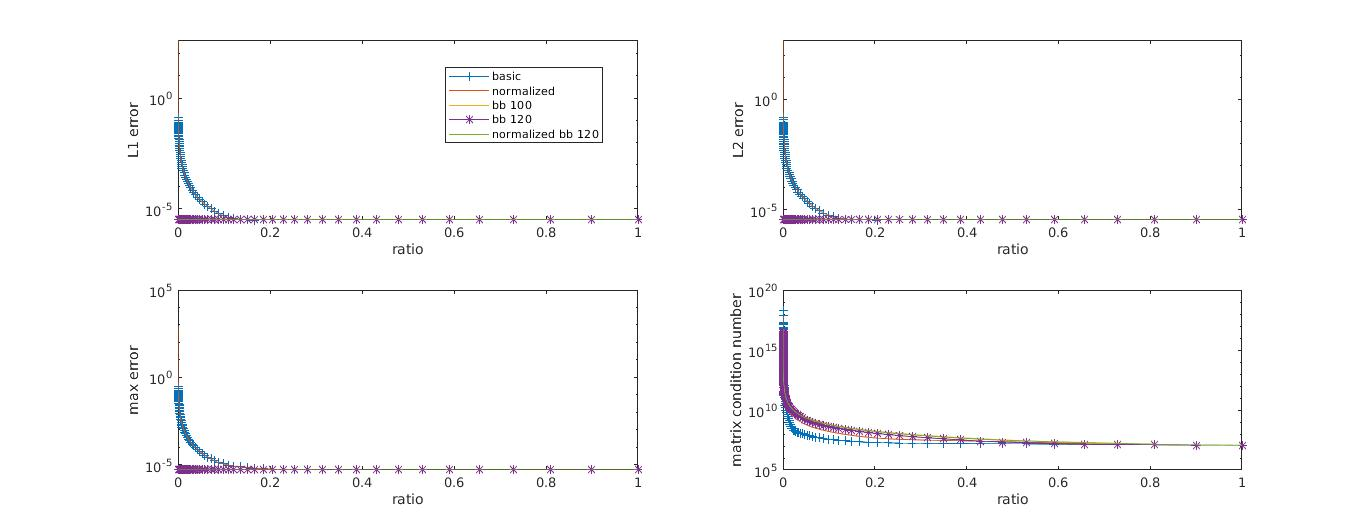
\includegraphics[width=\textwidth]{figure/cond_N2_prec1024.jpg}
 \caption{error and condition number by the interface position, polynomial 
degree 2, number of element 1024}
\end{figure}

\begin{figure}[hp!]
 \centering
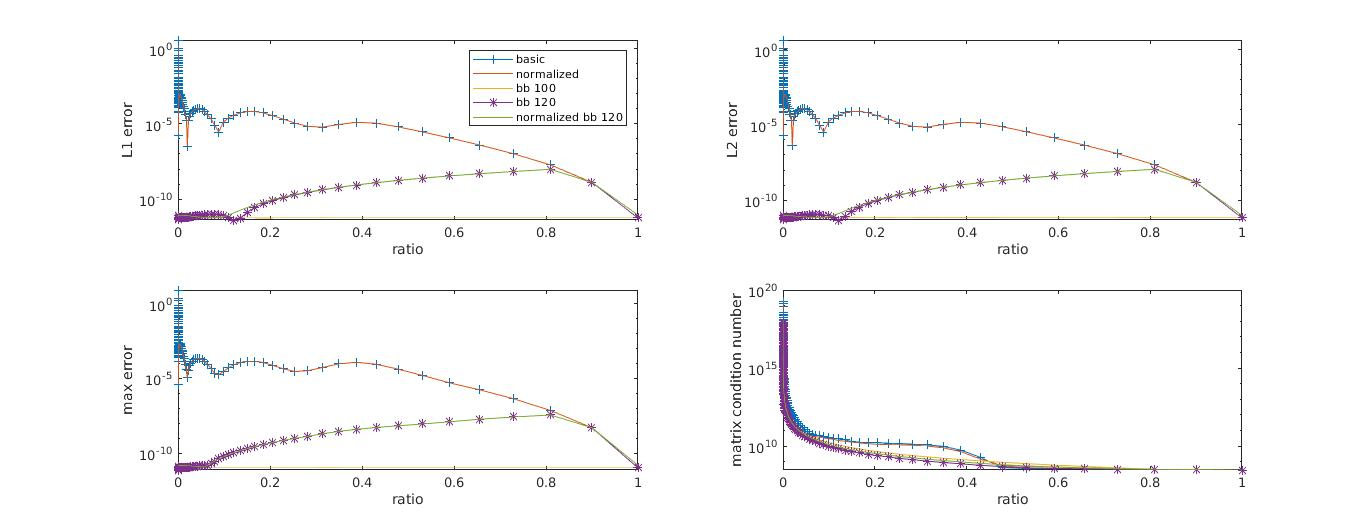
\includegraphics[width=\textwidth]{figure/cond_N6_prec1024.jpg}
 \caption{error and condition number by the interface position, polynomial 
degree 6, number of element 1024}
\end{figure}

We observe that every condition numbers increases in the same similar way. But 
we can see a big difference between the basic approach / normalized approach 
and the bounding box approach wich seems have better error results.

However, the methods does not seem to be high order method. For example, with 
7-order polynomials and a bounding box of $120\%$, the method order is $3.5$ 
average. There is no differences between the normalized and the basic method 
unless the higher matrix condition number in normalized method.

We also observed the effect of the size of the bounding box on the error and 
the conditionning number: we observe that larger the bounding box is, higher 
the error is, but lower the conditioning number is.

\begin{figure}[hb!]
 \centering
 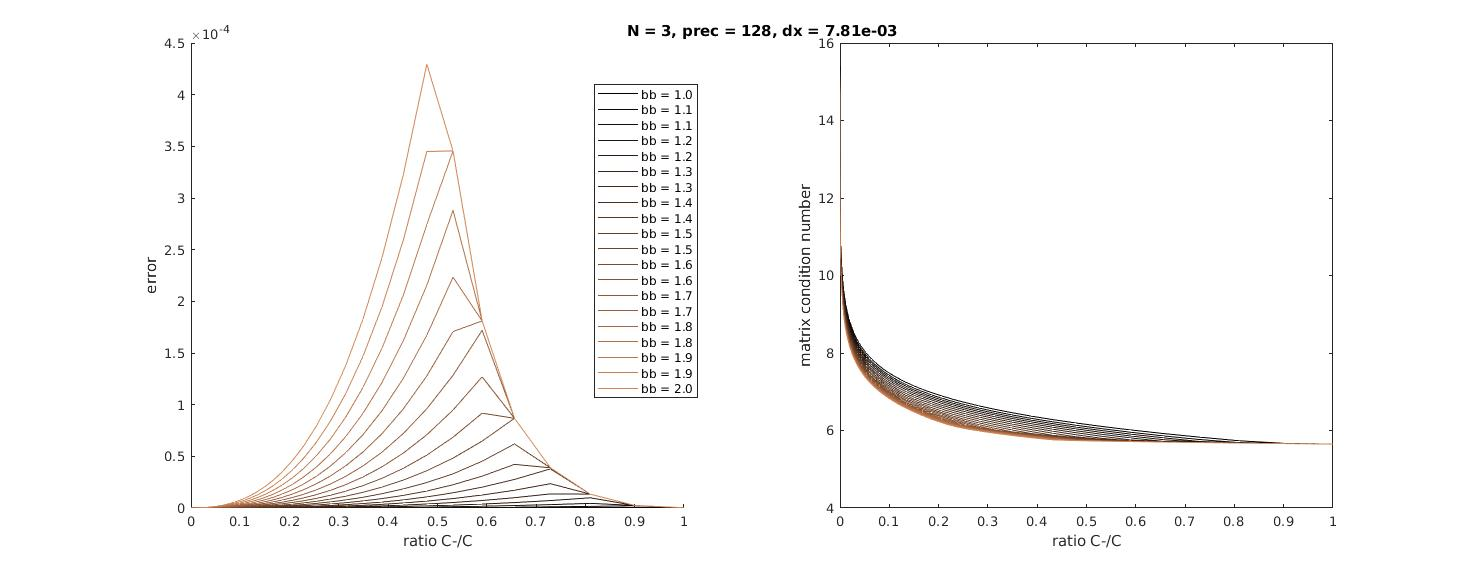
\includegraphics[width=\textwidth]{figure/bberror_N3_prec128.jpg}
 % bberror_N3_prec128.jpg: 1473x571 px, 72dpi, 51.96x20.14 cm, bb=0 0 1473 571
\end{figure}

\clearpage

\section{Coming back on the new approach}

We still look on the ratio $\dfrac{|\mathcal{C}^-|}{|\mathcal{C}|}$, but also 
on the mesh. We compare two subdivision generation method on an interval with 
an interface and a bounding box.

The interval of simulation is $]0,1[$ and the interval of interest is 
$]0,0.7[$. We create meshes with a bounding box of $120 \%$ on the edges. For 
example, if the original edge is $[0.5,1]$, then the bounding box process 
transforms this edge in $[0.5,0.94]$.

Here is a description of the two mesh generation processes:
\begin{enumerate}[label=(\alph*)]
 \item\label{process_a} We create a subdivision of $[0,1]$, then we prune 
the cells totaly 
outside of the interest interval. Finally, we compute the bounding box process 
on the cells containing the interface.
 \item\label{process_b} We create a subdivision of $[0,1]$, then we 
alternatively we prune 
the outside cells, we compute the bounding box process and either we divide all 
the cells into two cells and we repeat the previous process, or we stop the 
process because we have the precision needed.
\end{enumerate}

The two processes seems the same but it gives really differents results, as for 
the generated meshes than for the convergences results.

The following tables are two examples of the generated meshes:

% Please add the following required packages to your document preamble:
% \usepackage{multirow}
% \usepackage{graphicx}
\begin{table}[h!]
\centering
\caption{Meshes generated by process \ref{process_a} with an 
interface at $0.7$ and a $120\%$-bounding box.}
\resizebox{\textwidth}{!}{%
\begin{tabular}{|c|c|c|c|c|c|c|c|l|}
\hline
initial interval & \multicolumn{8}{c|}{{[}0,1{]}} \\ \hline
after bounding box & \multicolumn{8}{c|}{{[}0,0.84{]}} \\ \hline
dx & \multicolumn{8}{c|}{0.8400} \\ \hline
initial interval & \multicolumn{4}{c|}{\multirow{2}{*}{{[}0,0.5{]}}} & 
\multicolumn{4}{c|}{{[}0.5,1{]}} \\ \cline{1-1} \cline{6-9} 
after bounding box & \multicolumn{4}{c|}{} & \multicolumn{4}{c|}{{[}0.5,0.74{]}} 
\\ \hline
dx & \multicolumn{4}{c|}{0.5000} & \multicolumn{4}{c|}{0.2400} \\ \hline
initial interval & \multicolumn{2}{c|}{\multirow{2}{*}{{[}0,0.25{]}}} & 
\multicolumn{2}{c|}{\multirow{2}{*}{{[}0.25,0.5{]}}} & 
\multicolumn{2}{c|}{{[}0.5,0.75{]}} & \multicolumn{2}{c|}{pruned cell} \\ 
\cline{1-1} \cline{6-9} 
after bounding box & \multicolumn{2}{c|}{} & \multicolumn{2}{c|}{} & 
\multicolumn{2}{c|}{{[}0.5,0.74{]}} & 
\multicolumn{2}{c|}{\multirow{5}{*}{{[}0.75,1{]}}} \\ \cline{1-7}
dx & \multicolumn{2}{c|}{0.25} & \multicolumn{2}{c|}{0.25} & 
\multicolumn{2}{c|}{0.24} & \multicolumn{2}{c|}{} \\ \cline{1-7}
initial interval & \multirow{2}{*}{{[}0,0.125{]}} & 
\multirow{2}{*}{{[}0.125,0.25{]}} & \multirow{2}{*}{{[}0.25,0.375{]}} & 
\multirow{2}{*}{{[}0.375,0.5{]}} & \multirow{2}{*}{{[}0.5,0.625{]}} & 
{[}0.625,0.75{]} & \multicolumn{2}{c|}{} \\ \cline{1-1} \cline{7-7}
after bounding box &  &  &  &  &  & {[}0.625,0.715{]} & \multicolumn{2}{c|}{} \\ 
\cline{1-7}
dx & 0.1250 & 0.1250 & 0.1250 & 0.1250 & 0.1250 & 0.0900 & \multicolumn{2}{c|}{} 
\\ \hline
\end{tabular}%
}
\end{table}

% Please add the following required packages to your document preamble:
% \usepackage{multirow}
% \usepackage{graphicx}
\begin{table}[h!]
\centering
\caption{Meshes generated by process \ref{process_b} with an 
interface at $0.7$ and a $120\%$-bounding box.}
\label{tab:my-table}
\resizebox{\textwidth}{!}{%
\begin{tabular}{|c|c|c|c|c|c|c|c|c|}
\hline
initial interval & \multicolumn{8}{c|}{{[}0,1{]}} \\ \hline
after bounding box & \multicolumn{8}{c|}{{[}0,0.84{]}} \\ \hline
dx & \multicolumn{8}{c|}{0.84} \\ \hline
initial interval & \multicolumn{4}{c|}{\multirow{2}{*}{{[}0,0.42{]}}} & 
\multicolumn{4}{c|}{{[}0.42,0.84{]}} \\ \cline{1-1} \cline{6-9} 
after bounding box & \multicolumn{4}{c|}{} & 
\multicolumn{4}{c|}{{[}0.42,0.756{]}} \\ \hline
dx & \multicolumn{4}{c|}{0.42} & \multicolumn{4}{c|}{0.336} \\ \hline
initial interval & \multicolumn{2}{c|}{\multirow{2}{*}{{[}0,0.21{]}}} & 
\multicolumn{2}{c|}{\multirow{2}{*}{{[}0.21,0.42{]}}} & 
\multicolumn{2}{c|}{\multirow{2}{*}{{[}0.42,0.588{]}}} & 
\multicolumn{2}{c|}{{[}0.588,0.756{]}} \\ \cline{1-1} \cline{8-9} 
after bounding box & \multicolumn{2}{c|}{} & \multicolumn{2}{c|}{} & 
\multicolumn{2}{c|}{} & \multicolumn{2}{c|}{{[}0.588,0.7224{]}} \\ \hline
dx & \multicolumn{2}{c|}{0.21} & \multicolumn{2}{c|}{0.21} & 
\multicolumn{2}{c|}{0.168} & \multicolumn{2}{c|}{0.1344} \\ \hline
initial interval & \multirow{2}{*}{{[}0,0.105{]}} & 
\multirow{2}{*}{{[}0.105,0.21{]}} & \multirow{2}{*}{{[}0.21,0.315{]}} & 
\multirow{2}{*}{{[}0.315,0.42{]}} & \multirow{2}{*}{{[}0.42,0.504{]}} & 
\multirow{2}{*}{{[}0.504,0.588{]}} & \multirow{2}{*}{{[}0.588,0.6552{]}} & 
{[}0.6552,0.756{]} \\ \cline{1-1} \cline{9-9} 
after bounding box &  &  &  &  &  &  &  & {[}0.6552,0.709{]} \\ \hline
dx & 0.105 & 0.105 & 0.105 & 0.105 & 0.084 & 0.084 & 0.0672 & 0.0538 \\ \hline
\end{tabular}%
}
\end{table}

We observe two major differences between the two methods:
\begin{itemize}
 \item The second method has no pruned cell, and therefore, the number of cell 
is always $2^{\text{depth}}$.
\item The cell widths has not the same monotony properties: let be $D$ the 
depth, $dx_i^D$ for the width of the initial interval, and $dx_b^D$ the cell 
width after the bounding box process. The important width we want to control is 
$dx_b$. Then, with the process \ref{process_a}, $dx_b^D \leq \dfrac{1}{2} 
dx_i^{D-1}$ whereas the process \ref{process_b} gives $dx_b^D \leq \dfrac{1}{2} 
dx_b^{D-1}$ which is better.
\end{itemize}

We can easily very bad cases where we have actualy no control, for example if 
we put the interface at $0.5+\epsilon$. Then the final cell will always be 
$[0.5,0.5+1.2\epsilon]$, wich is really bad because we cannot make any 
refinment in the interface region.

The results are obvious:

\begin{figure}[hp!]
\begin{subfigure}[t]{0.45\textwidth}
 \centering
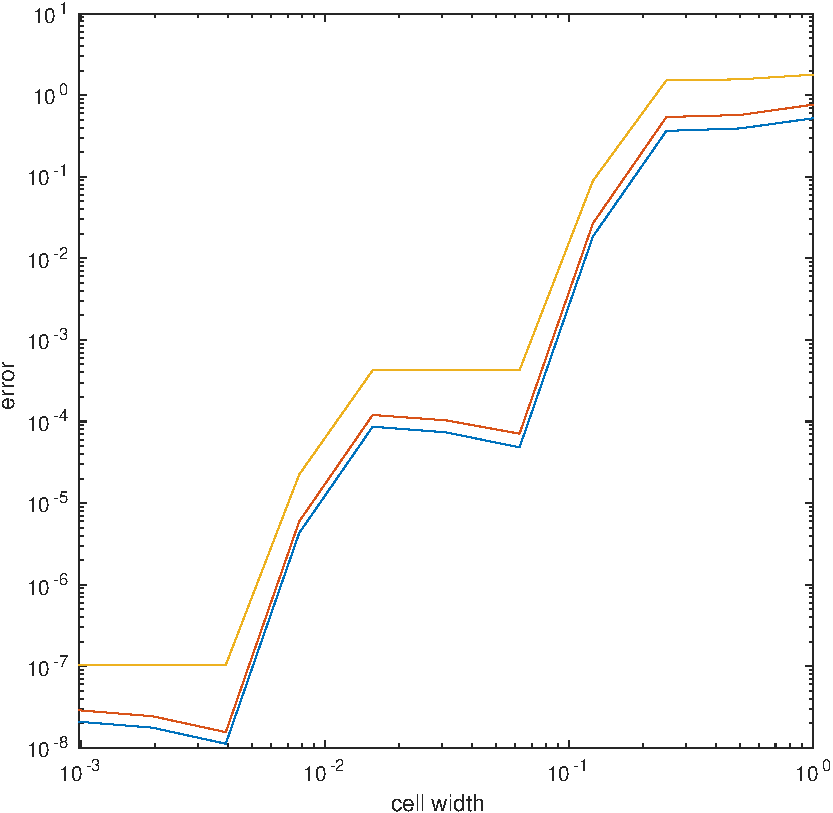
\includegraphics[width=\textwidth]{figure/poisson_error-eps-converted-to.pdf}
 \caption{convergence result with the process \ref{process_a}, with an average 
order of 3.75. }
\end{subfigure}
\hfill
\begin{subfigure}[t]{0.45\textwidth}
 \centering
 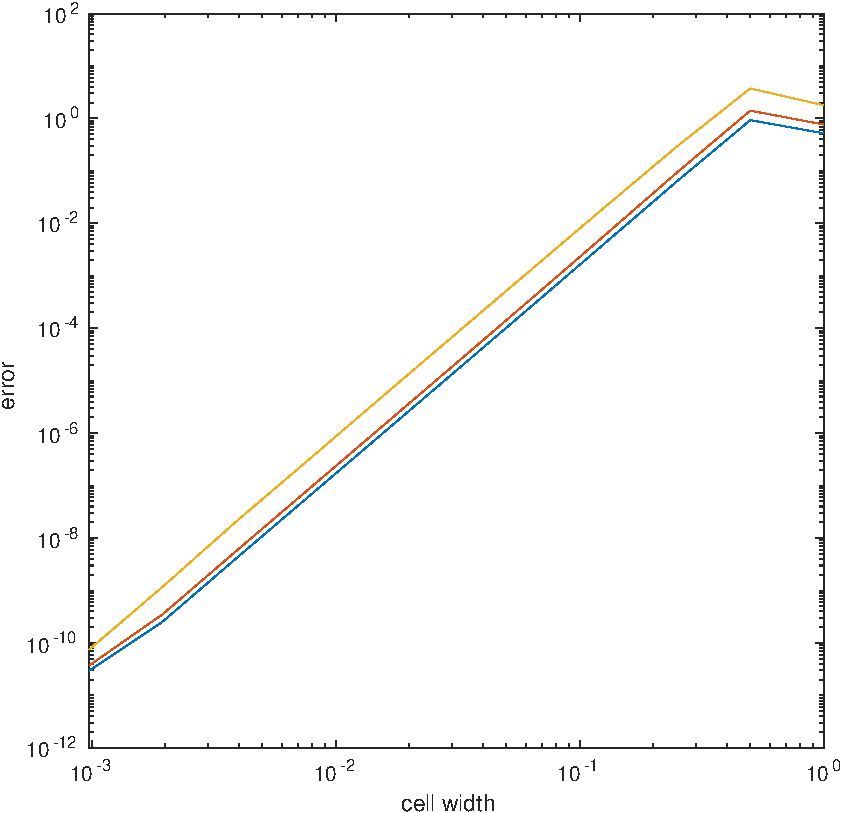
\includegraphics[width=\textwidth] 
{figure/poisson_error_stabilized-eps-converted-to.pdf}
 \caption{convergence result with the process \ref{process_a}, with an average 
order of 3.96. }
\end{subfigure}
\caption{Convergence comparison}
\end{figure}

In 1D, the processes seems quite similar, but in 2D, the differences are 
obvious:

\begin{figure}[hp!]
\input{tikz/sample.tikzstyles}
\ctikzfig{tikz/test}
\caption{The two meshes generation method}
\end{figure}
% Please add the following required packages to your document preamble:
% \usepackage{graphicx}
\begin{table}[hp!]
\centering
\caption{Convergence table}
\label{tab:my-table}
\resizebox{\textwidth}{!}{%
\begin{tabular}{|c|c|c|c|c|c|c|c|c|c|c|c|}
\hline
polynomial order & 0 & 1 & 2 & 3 & 4 & 5 & 6 & 7 & 8 & 9 & 10 \\ \hline
convergence order & 1.13 & 2.19 & 2.06 & 3.97 & 4.01 & 3.87 & 3.96 & 3.96 & 3.98 
& 3.96 & 4.01 \\ \hline
\end{tabular}%
}
\end{table}


\end{document}
